\documentclass[preview]{standalone}
\usepackage{anyfontsize}
\usepackage{t1enc}
\usepackage{amsmath}
\usepackage{tcolorbox}
\usepackage{tikz}
\usepackage{amsfonts}
\usepackage{graphicx}
\usepackage{fancyhdr}
\usepackage{clrscode}
\usepackage{extramarks}
\usepackage{enumerate}
\usepackage{tkz-graph}
\usepackage[utf8]{inputenc}
\usetikzlibrary{shapes.geometric,arrows,automata,matrix,shapes,arrows,positioning,chains}

% golang colors
\definecolor{blue}{RGB}{55,94,171}
\definecolor{lblue}{RGB}{224,235,245}

% default sans
\renewcommand{\familydefault}{\sfdefault}

%%\fontencoding{T1}
%\fontfamily{calibri}
%%\fontseries{m}
%%\fontshape{it}
%\fontsize{28}{28}
%\selectfont

% deprecated -- use tikzset
\tikzstyle{process} = [rectangle,
minimum width=2cm, minimum height=1.8cm,
text width=3.6cm, text centered,
draw=blue, fill=lblue]

\tikzstyle{arrow} = [ultra thick, ->, >=latex]

\tikzset{
    block/.style={
        rectangle, rounded corners=0.1cm,
        minimum width=2cm, minimum height=1.8cm,
        text width=3.6cm, text centered,
        draw=blue, fill=lblue
    },
    invis/.style={
        draw=white
    },
    descr/.style={
        fill=white,
        inner sep=2.5pt
    },
    connector/.style={
        very thick,
        -latex,
        font=\scriptsize
    },
    rectangle connector/.style={
        connector,
        to path={(\tikztostart) -- ++(#1,0pt) \tikztonodes |- (\tikztotarget) },
        pos=0.5
    },
    rectangle connector/.default=-2cm,
    straight connector/.style={
        connector,
        to path=--(\tikztotarget) \tikztonodes
    }
}


\begin{document}
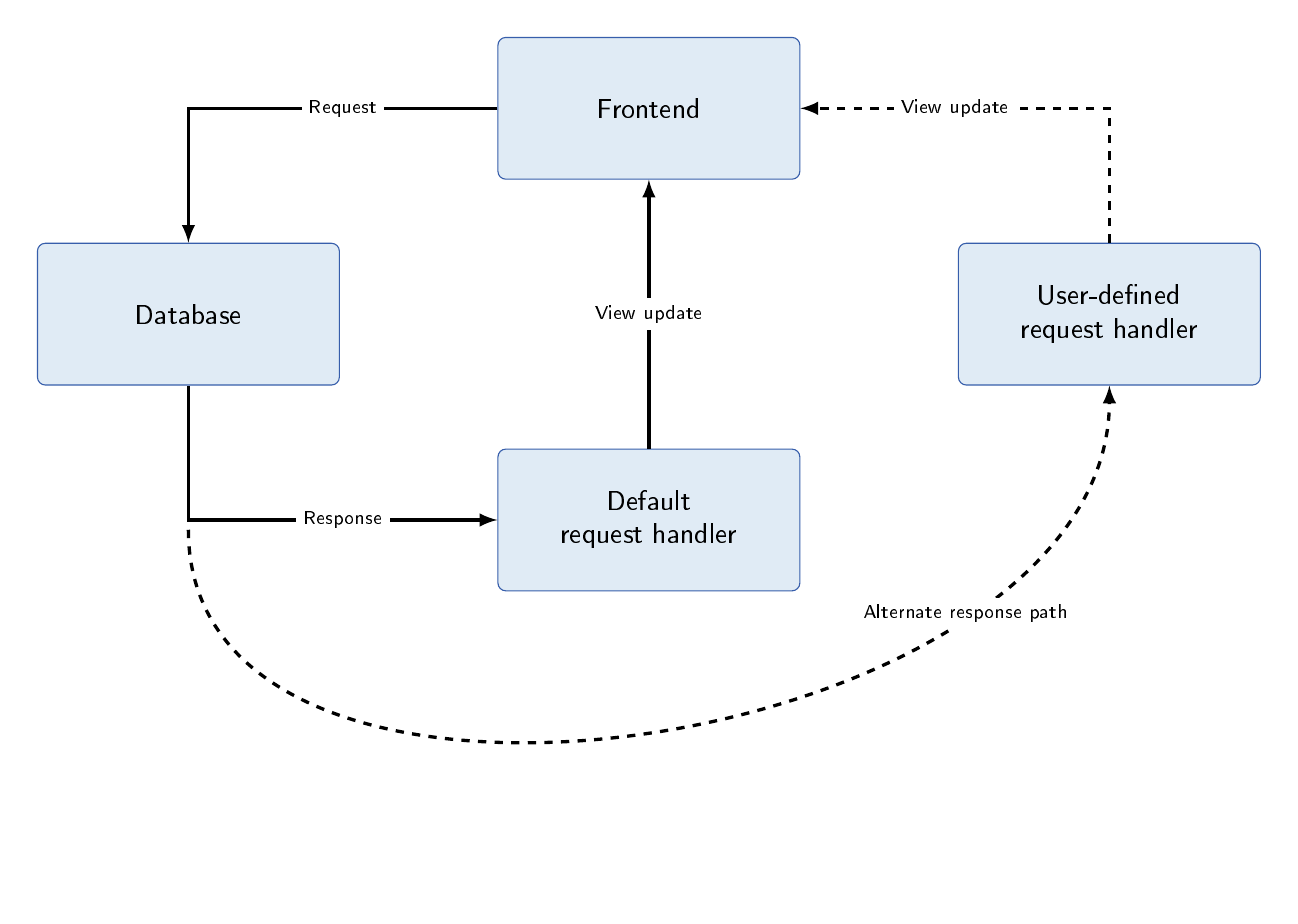
\begin{tikzpicture}[node distance=4cm]
    \matrix (m)[matrix of nodes,
    column sep=2cm,row sep=8mm,
    align=center, nodes={rectangle,draw, anchor=center}] {
        &   |[block]| {Frontend}   &               \\
        |[block]| {Database}    &   &   |[block]| {User-defined \\ request handler}  \\
        |[invis]| &   |[block]| {Default \\ request handler}   &               \\
    };
    \draw [connector] (m-1-2) -| node[descr, pos=0.25] {Request} (m-2-1);
    \draw [connector] (m-2-1) |- node[descr, pos=0.75] {Response} (m-3-2);
    \draw [connector] (m-3-2) -> node[descr, pos=0.50] {View update} (m-1-2);
    \draw [connector, dashed] (m-2-3) |- node[descr, pos=0.75] {View update} (m-1-2);
    \draw [connector=-3cm,dashed,relative=false,out=270,in=270]
        (m-3-1) edge node[descr, pos=0.75] {Alternate response path} (m-2-3);
\end{tikzpicture}
\end{document}
